%************************************************
\chapter{Motivación e Introducción}\label{ch:introduction}
% ************************************************

\section{¿Qué es el Procesamiento del Lenguaje Natural?}
\label{sec:whatisnlp}

El lenguaje natural se refiere a cualquier lenguaje hablado por un humano, (\eg
Inglés, Castellano o Chino). El \ac{NLP}\marginpar{\acf{PNL}} es un campo de la
ciencia de la computación e ingeniería desarrollado a partir del estudio del
lenguaje y la computación lingüistica dentro del campo de la \ac{IA}. Los
objetivos del \ac{NLP} son diseñar y construir aplicaciones que faciliten la
interacción humana con la máquinas y otros dispositivos mediante el uso del
lenguaje natural. Dentro del amplio campo del \ac{NLP} podemos distinguir las
siguientes áreas principales:

\begin{description}\label{sec:nlpfields}
  \item[QAS:] \ac{QAS}\marginpar{\acf{SRA}}. En estos sistemas se pretende
    remplazar a los usuales buscadores en los que introducimos un texto para
    obtener algún tipo de respuesta a una pregunta. Por ejemplo, si quisieramos
    saber a qué hora abre un centro comercial, bastaría con hablarle al sistema
    en lenguaje natural -- nuestro lenguaje natural, ya sea Inglés, Alemán o
    Castellano y el sistema nos daría respuesta a nuestra pregunta. Aunque ya
    existen este tipo de sistemas (\eg \emph{Siri, Cortana\dots}) están aún en
    una situación muy precaria, ya que ninguno entiende por completo el lenguaje
    natural, solo un subconjunto de frases clave.
  \item[Resúmenes:] Este área incluye aplicaciones que puedan, basándose en una
    colección de documentos, dar como salida un resumen coherente del contenido
    de los mismos. Otra de las posibles aplicaciones sería generar
    presentaciones a partir de dichos documentos.
  \item[Traducción:] Esta fue la principal área de investigación en el campo del
    \ac{NLP}. Como claro ejemplo tenemos el traductor de Google, mejorando día a
    día. Sin embargo, un traductor realmente útil sería aquel que consiga
    traducir en tiempo real una frase que le dictemos mientras decidimos qué
    línea de autobús debemos coger para llegar a tiempo a una conferencia en
    Zurich.
  \item[Reconocimiento de voz:] Una de las tareas más difíciles en \ac{NLP}. Aún
    así, se han conseguido grandes avances en la construcción de modelos que
    pueden usarse en el teléfono móvil o en el ordenador. Estos modelos son
    capaces de reconocer expresiones del lenguaje hablado como preguntas y
    comandos. Desafortunadamente, los sistemas \ac{ASR}\marginpar{\acf{RVA}}
    funcionan bajo dominios muy acotados y no permiten al interlocutor desviarse
    de la entrada que espera el sistema, \eg \emph{``Por favor, diga ahora la
      opción a elegir: 1 Para\dots, 2 para\dots''}
  \item[Clasificación de documentos:] Una de las áreas más exitosas del
    \ac{NLP}, cuyo objetivo es identificar a qué categoría debería pertenecer un
    documento. Ha demostrado tener un amplio abanico de aplicaciones, \eg
    filtrado de \emph{spam}, clasificación de artículos de noticias,
    valoraciones de películas\dots Parte de su éxito e impacto se debe a la
    facilidad relativa que conlleva entrenar los modelos de aprendizaje para
    hacer dichas clasificaciones.
\end{description}

El \ac{NLP} emplea técnicas computacionales con el propósito de aprender,
entender y producir lenguaje humano. Las aproximaciones de hace unos años en el
campo de la investigación del lenguaje se centraban en automatizar el análisis
de las estructuras lingüísticas y desarrollar tecnologías como las mencionadas
anteriormente. Los investigadores de hoy en día se centran en usar dichas
herramientas en aplicaciones para el mundo real, creando sistemas de diálogo
hablados y motores de traducción \emph{Speech-to-Speech}, es decir, dados dos
interlocutores, interpretar y traducir sus frases. Otro de los focos en los que
se centran las investigaciones actuales son la minería en redes sociales en
busca de información sobre salud, finanzas e identificar los sentimietos y
emociones sobre determinados productos. 

\section{Historia del Procesamiento del Lenguaje Natural}
\label{sec:currentnlp}

A continuación, citamos algunos de los avances en este campo durante los últimos
años según \citet{Hirschberg2015}.

Durante las primeras épocas de esta ciencia, se intentaron escribir vocabularios
y reglas del lenguaje humano para que el ordenador las entendiera. Sin embargo,
debido a la naturaleza ambigua, variable e interpretación dependiente del
contexto de nuestro lenguaje resultó una ardua tarea. Por ejemplo, una estrella
puede ser un ente astronómico o una persona, y puede ser un nombre o un verbo.

En la década de los 90, los investigadores transformaron el mundo del \ac{NLP}
desarrollando modelos sobre grandes cantidades de datos sobre lenguajes. Estas
bases de datos se conocen como \emph{corpus}. El uso de estos conjuntos de datos
fueron uno de los primeros éxitos notables del uso del \emph{big data}, mucho
antes de que el \ac{AA} acuñara este término.

Esta aproximación estadística al \ac{NLP} descubrió que el uso de métodos
simples usando palabras, secuencias del \emph{\ac{POS}}\marginpar{\ac{POS}: Categorías
  morfosintácticas en castellano} (si una palabra es un nombre, verbo o
preposición), o plantillas simples pueden obtener buenos resultados cuando son
entrenados sobre un gran conjunto de datos. A día de hoy, muchos sistemas de
clasificación de texto y sentimientos se basan únicamente en los distintos
conjuntos de palabras o \emph{``bag of words''} que contienen los documentos,
sin prestar atención a su estructura o significado. El estado del arte de hoy
día usa aproximaciones con \ac{AA} y un rico conocimiento de la estructura
lingüística. Un ejemplo de estos sistemas es \emph{Stanford CoreNLP}
\citep{Manning2014}. \emph{CoreNLP} proporciona un \emph{pipeline} estándar para
el procesamiento del \ac{NLP} incluyendo:

\begin{description}
  \item[POS Tagging:] o etiquetado morfosintáctico. Módulo encargado de leer
    texto en algún lenguaje y asignar la categoría morfosintáctica a cada
    palabra, \eg nombre, verbo, adjetivo\dots aunque por lo general se suelen
    usar etiquetas más detalladas como ``\emph{nombre-plural}''.
  \item[NER:] \ac{NER}, etiqueta palabras en un texto correspondientes a
    \emph{nombres de cosas}, como personas, nombres de compañías, nombres de
    proteínas o genes etc. En concreto, \emph{CoreNLP} distingue de forma muy
    precisa tres tipos de clases, personas, organizaciones y localizaciones.
  \item[Parseo Gramatical:] Resuelve la estructura gramatical de frases, \eg qué
    grupos de palabras van juntos formando frases y qué palabras son sujeto u
    objeto de un verbo. Como se ha comentado, en aproximaciones anteriores se
    usaban parseadores probabilísticos usando conocimiento del lenguaje a partir
    de sentencias analizadas sintácticamente a mano. Para así producir el
    análisis más probable de sentencias nuevas. Actualmente se se usan
    parseadores estadísticos, los cuales aún comenten fallos, pero funcionan
    bien a rasgos generales.
  \item[DP:] \ac{DP} o parseo de dependencias. Analiza la estructura gramatical
    de una frase, estableciendo relaciones entre palabras principales y palabras
    que modifican dichas palabras principales. La \autoref{fig:nndep} muestra un
    ejemplo. La flecha dirigida de la palabra \emph{moving} a la palabra
    \emph{faster} indica que \emph{faster} modifica a \emph{moving}. La flecha
    está etiquetada con una palabra, en este caso \emph{advmod}, indicando la
    naturaleza de esta dependencia. La \autoref{fig:corenlp} muestra ejemplos de
    los distintos módulos del \emph{pipeline} de \emph{CoreNLP}
\end{description}

\begin{figure}[bth]
  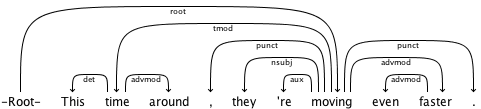
\includegraphics[width=1\linewidth]{gfx/nndep-example}
  \caption[Ejemplo de parseo de dependencias]{Ejemplo de parseo de dependencias}
  \label{fig:nndep}
\end{figure}

\begin{figure}[bth]
  \makebox[\textwidth][c]{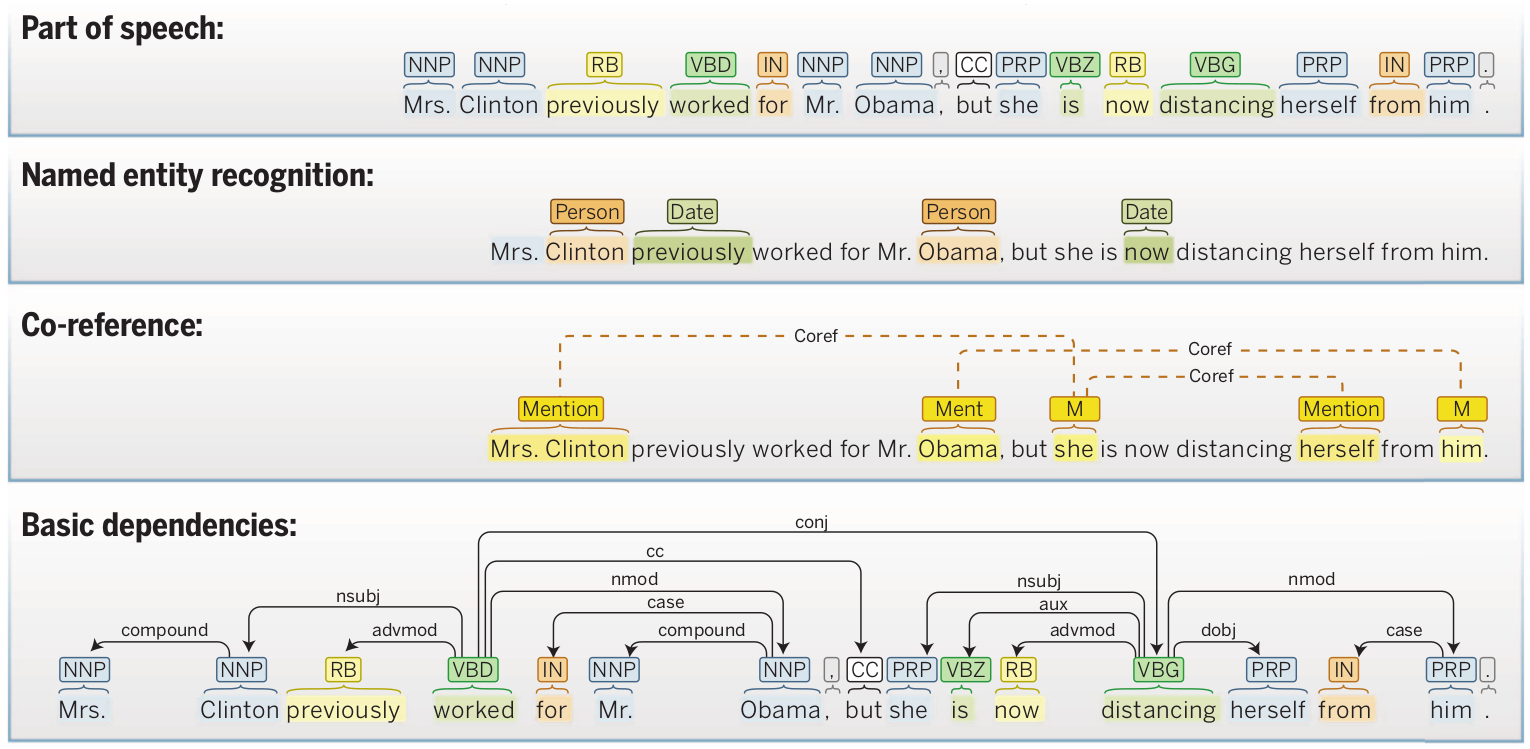
\includegraphics[width=1.5\textwidth]{gfx/corenlp}}
  \caption[Ejemplo de parseo de dependencias]{Many language technology tools start by doing linguistic structure analysis. Here we show output from Stanford CoreNLP. As shown from top to
bottom, this tool determines the parts of speech of each word, tags various words or phrases as semantic named entities of various sorts, determines which entity
mentions co-refer to the same person or organization, and then works out the syntactic structure of each sentence, using a dependency grammar analysis.}
  \label{fig:corenlp}
\end{figure}

\section{Limitaciones}
\label{sec:nlplimits}

Aunque se han producido avances, una de las principales limitaciones del
\ac{NLP} hoy día es el hecho de que la mayoría de recursos y sistemas solo están
disponibles para los denominados \acp{HRL}\marginpar{\ac{HRL}: Idiomas de altos
recursos}, estos lenguajes son el Inglés, Francés, Español, Alemán y Chino. Por
contra, hay una gran cantidad de \acp{LRL} --\marginpar{\ac{LRL}: Idiomas de bajos
recursos} como Bengalí, Indonesio, Punjabí, Cebuano y Swahili -- hablados y
escritos por millones de personas que no disponen de este tipo de sistemas. Uno
de los mayores retos para la comunidad del lenguaje es desarrollar recursos y
herramientas para cientos o miles de lenguajes, no solo para unos pocos.


